\documentclass[handout, serif, aspectratio=169, 10pt]{beamer}

% packages
%\usepackage{newpxmath} % math font is Palatino compatible
%\usepackage[nomath]{fontspec}

\usepackage{setspace}
\usepackage{xcolor}
\usepackage{soul} % for \st
\usepackage{hyperref} % for links
\definecolor{links}{HTML}{2A1B81}
\hypersetup{colorlinks,linkcolor=,urlcolor=links}


% table stuff
\usepackage{chronosys}
\usepackage{verbatim}
% \pagenumbering{arabic}
\usepackage{tabularx}
\usepackage{booktabs}
\usepackage{ragged2e}
\usepackage{mathtools}

% R Code
\usepackage{listings}
\usepackage{courier}
\lstset{basicstyle=\scriptsize\ttfamily,breaklines=true}
\lstset{framextopmargin=50pt,frame=bottomline}

% themes
\usetheme[progressbar=frametitle, block=fill]{metropolis}
\useoutertheme{metropolis}
\useinnertheme{metropolis}

% colors
\definecolor{dimwhite}{rgb}{0.99, 0.99, 0.99}
\definecolor{charcoal}{rgb}{0.21, 0.27, 0.31}
\definecolor{slategray}{rgb}{0.44, 0.5, 0.56}
\definecolor{dimgray}{rgb}{0.41, 0.41, 0.41}
\definecolor{bleudefrance}{rgb}{0.19, 0.55, 0.91}

% beamer options
\setbeamercolor{author}{fg=charcoal}
\setbeamercolor{background canvas}{bg=white}
\setbeamercolor{section in toc}{fg=charcoal}
\setbeamercolor{subsection in toc}{fg=dimgray}
\setbeamercolor{frametitle}{bg=dimwhite, fg=charcoal}
\setbeamercolor{progress bar}{fg=slategray, bg=fg!50!black!30}
\setbeamercovered{transparent}
\setbeamertemplate{itemize items}[triangle]
\setbeamertemplate{itemize subitem}[circle]
\setbeamertemplate{itemize subsubitem}[square]
\setbeamersize{text margin left=7mm,text margin right=7mm} 

% new commands
\newcommand{\q}[1]{``#1''}
\newcommand{\hs}[1]{\textsc{\hfill\scriptsize\color{dimgray}#1}}
\newcommand{\g}[1]{{\color{gray}#1}}
\newcommand{\dg}[1]{{\color{dimgray}#1}}
\newcommand{\sg}[1]{{\color{slategray}#1}}
\newcommand{\bdf}[1]{{\color{bleudefrance}#1}}
\newcommand{\itemcolor}[1]{\renewcommand{\makelabel}[1]{\color{#1}\hfil ##1}}
\newcommand\Wider[2][2em]{
\makebox[\linewidth][c]{
  \begin{minipage}{\dimexpr\textwidth+#1\relax}
  \raggedright#2
  \end{minipage}
  }
}

% misc
\linespread{1.35}

% Math stuff
\newcommand{\norm}[1]{\left\lVert#1\right\rVert}
\newcommand{\R}{\mathbb{R}}
\newcommand{\E}{\mathbb{E}}
\newcommand{\V}{\mathbb{V}}
\newcommand{\probP}{\mathbb{P}}
\newcommand{\ol}{\overline}
%\newcommand{\ul}{\underline}
\newcommand{\pp}{{\prime \prime}}
\newcommand{\ppp}{{\prime \prime \prime}}
\newcommand{\policy}{\gamma}
\newcommand{\plim}{ \overset{p}{\to}}
\newcommand{\hnot}{ \overset{H_0}{\to}}

% Causal Graphs
\usetikzlibrary{shapes,decorations,arrows,calc,arrows.meta,fit,positioning}
\tikzset{
    -Latex,auto,node distance =1 cm and 1 cm,semithick,
    state/.style ={ellipse, draw, minimum width = 0.7 cm},
    point/.style = {circle, draw, inner sep=0.04cm,fill,node contents={}},
    bidirected/.style={Latex-Latex,dashed},
    el/.style = {inner sep=2pt, align=left, sloped}
}

\title [Nonparametrics]{Nonparametrics and Local Methods: Splines}
\author{C.Conlon}
\institute{Applied Econometrics}
\date{\today}
\setbeamerfont{equation}{size=\tiny}
\begin{document}

\begin{frame}
\titlepage
\end{frame}
\begin{frame}{Polynomial Basis}
Again consider the following relationship:
\begin{align*}
y_i = f(x_i) + \epsilon_i
\end{align*}
One approach is to approximate $f(x_i)$ or $\E[y_i | x_i]$ with a \alert{polynomial series}.
\begin{align*}
y_i = a_0^k  + a_1^k x_i + a_2^k x_i^2 + a_3^k x_i^3+ \varepsilon_i \text{ for } x \in [\underline{x}_k,\overline{x}_k]
\end{align*}
New idea: approximate $f(x_i)$ with \alert{different functions} at different intervals of $ [\underline{x}_k,\overline{x}_k]$.\\
Hard part: maintain that $\hat{f}(x_i)$ is twice continuously differentiable...
\end{frame}


\begin{frame}{Splines}
Splines are piecewise interpolating functions
\begin{definition} 
A function $s(x)$ on $[lb,ub]$ is a spline of order $m$ IFF
\begin{enumerate}
\item $s$ is $\mathbb{C}^{m-2}$ on $[lb,ub]$ and 
\item there is a grid of points (nodes) $lb = x_0 < x_1 < \cdots < x_k = ub$ such that $s(x)$ is a polynomial of degree $m-1$ on each subinterval $[x_k, x_{k+1}]$, $k = 0,\ldots,K-1$
\end{enumerate}
\end{definition}
Second order $(m=2)$ is piecewise linear.\\
We usually use cubic splines.
\end{frame}


\begin{frame}{Cubic Splines}
\small
\begin{itemize}
\item Lagrange data set $(x_i,y_i)$ for $i=0,\ldots n$.
\item Nodes: the $x_i$ are the nodes of the spline
\item Functional form $s(x) = a_i + b_i x + c_i x^2 + d_i x^3$ on $[x_{i-1},x_i]$
\item Unknowns $4n$ unknown coefficients
\item $2n$ interpolation and continuity conditions:
\begin{eqnarray*}
y_i &=& a_i + b_i x_i + c_i x_i^2 + d_i x_i^3 \quad i=1,\dots, n\\
y_i &=& a_{i+1} + b_{i+1} x_i + c_{i+1} x_i^2 + d_{i+1} x_i^3 \quad i=0,\ldots, n-1
\end{eqnarray*}
\item $2n - 2$ conditions from $\mathbb{C}^2$ at the interior for $i=1,\ldots,n-1$
\begin{eqnarray*}
b_i + 2c_i x_i + 3 d_i x_i^2  &=& b_{i+1} + 2 c_{i+1} x_i + 3 d_{i+1}x_i^2\\ 
2c_i + 6d_i x_i &=& 2c_{i+1} + 6d_{i+1} x_i
\end{eqnarray*}
\end{itemize}
\end{frame}


\begin{frame}{Side Conditions}
We have $4n-2$ linear equations and $4n$ unknowns we need two side conditions to identify the system
\begin{itemize}
\item Natural spline: $s''(x_0) = s''(x_n) = 0$ minimizes the total curvature $\int_{x_0}^{x_n} s''(x)^2 dx$
\item Hermite spline: $s'(x_0) = y_0'$ and $s'(x_n) = y_n'$ (with extra data)
\item Secant Hermite: $s'(x_0) = \frac{s(x_1) - s(x_0)}{x_1-x_0}$ , $s'(x_n) = \frac{s(x_n) - s(x_{n-1})}{x_n-x_{n-1}}$
\item Solvers are built in to packages like R (check documentation for which method).
\end{itemize}
\end{frame}


\begin{frame}{Shape Issues}
\begin{figure}[htbp]
\begin{center}
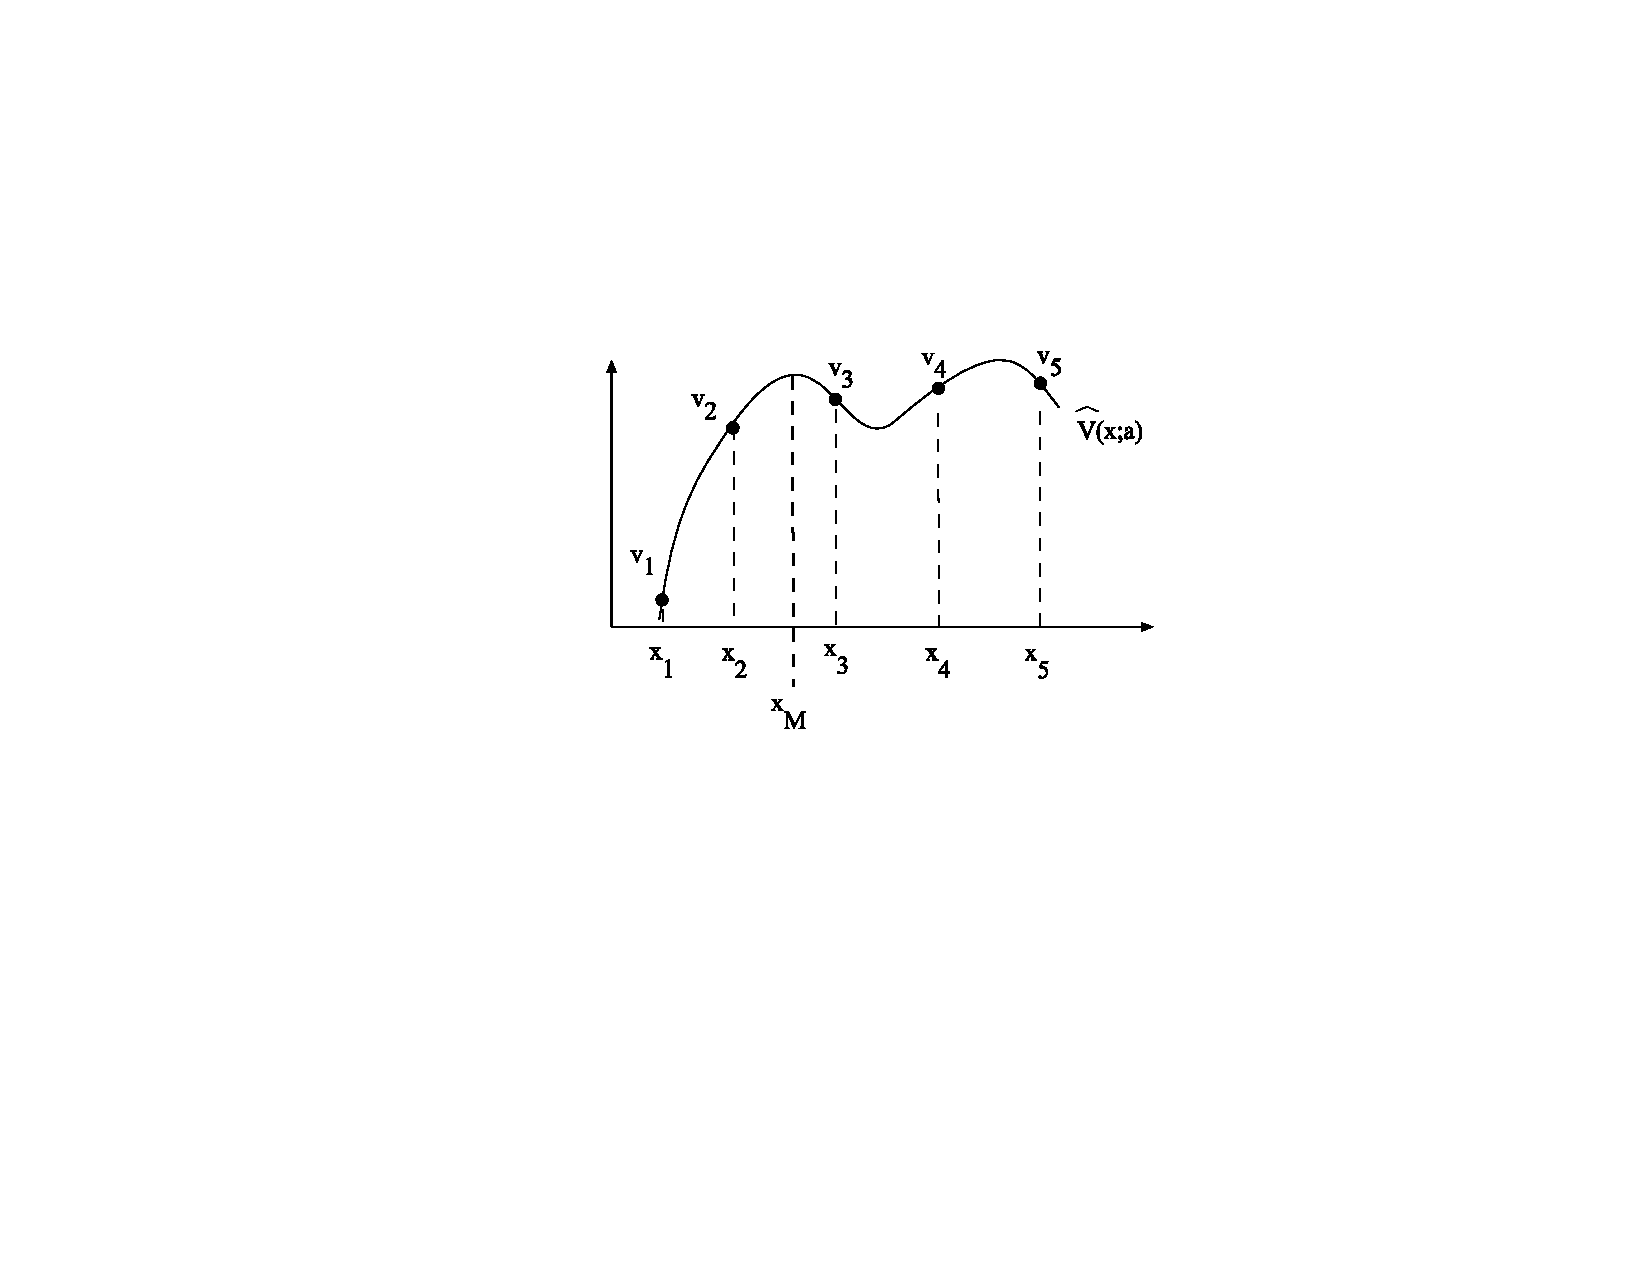
\includegraphics[height=2in]{./resources/spline_textbook.pdf}
\label{default}
\end{center}
\end{figure}
\begin{itemize}
\item Concave (monotone) data may lead to non concave (non monotone) approximations
\end{itemize}
\end{frame}

\begin{frame}{Schumaker Procedure (Shape Preserving Splines)}
\begin{enumerate}
\item Take level (and maybe slope) data at nodes $x_k$
\item Add intermediate nodes $z_k^{+} \in [x_k,x_{k+1}]$
\item Run quadratic spline with nodes at the $x$ and $z$ nodes which interpolate data and preserves shape
\item Schumaker formulas tell you how to choose the $z$ and spline coefficient
\item Detail in Judd and in companion paper (Judd and Solnick)
\end{enumerate}
\end{frame}

\begin{frame}[fragile]{Spline Example}
\begin{columns}
\begin{column}{0.5\textwidth}
\begin{itemize}
\item Try two piecewise cubics (at $x=3$)
\item Try three piecewise cubics (at $x=(2,4)$)
\item Try single cubic
\end{itemize}

 \tiny
 \vspace{2.4cm}
\begin{verbatim}
library(splines)
ggplot(data=NULL,aes(x, y)) + geom_point() + 
  geom_smooth(method = "lm", formula = y ~ bs(x,knots=3) ,color='maroon')+
  geom_smooth(method = "lm", formula = y ~ bs(x,knots=c(2,4)) ,color='darkgreen')+
  geom_smooth(method = "lm", formula = y ~ poly(x, 3),color='navy')
\end{verbatim}
\end{column}
\begin{column}{0.5\textwidth}  %%<--- here
    \begin{center}
    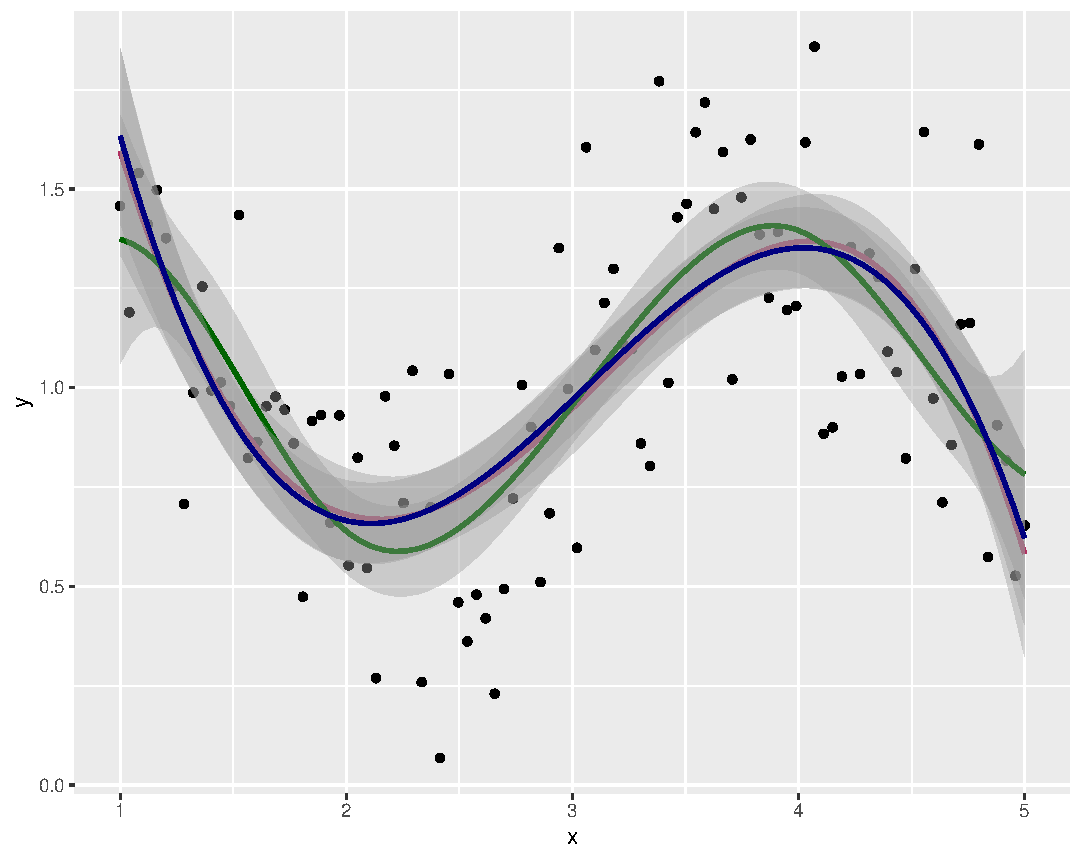
\includegraphics[width=\textwidth]{./resources/splines.pdf}
     \end{center}
\end{column}
\end{columns}
\end{frame}



\begin{frame}[fragile]{Spline Example}
\begin{itemize}
\item Alternative is to use \alert{generalized additive model} and fit a spline with the \texttt{s()} function.
\item These can be made quite flexible (but this is simple).
\end{itemize}
 \tiny
\begin{verbatim}
library(mgcv)
ggplot(data=NULL,aes(x, y)) + geom_point() + 
  geom_smooth(method = "lm", formula = y ~ bs(x,knots=3) ,color='maroon')+
  stat_smooth(method = gam, formula = y ~ s(x),color='navy')
\end{verbatim}
\end{frame}


  
  
\begin{frame}{My own example}
\begin{center}
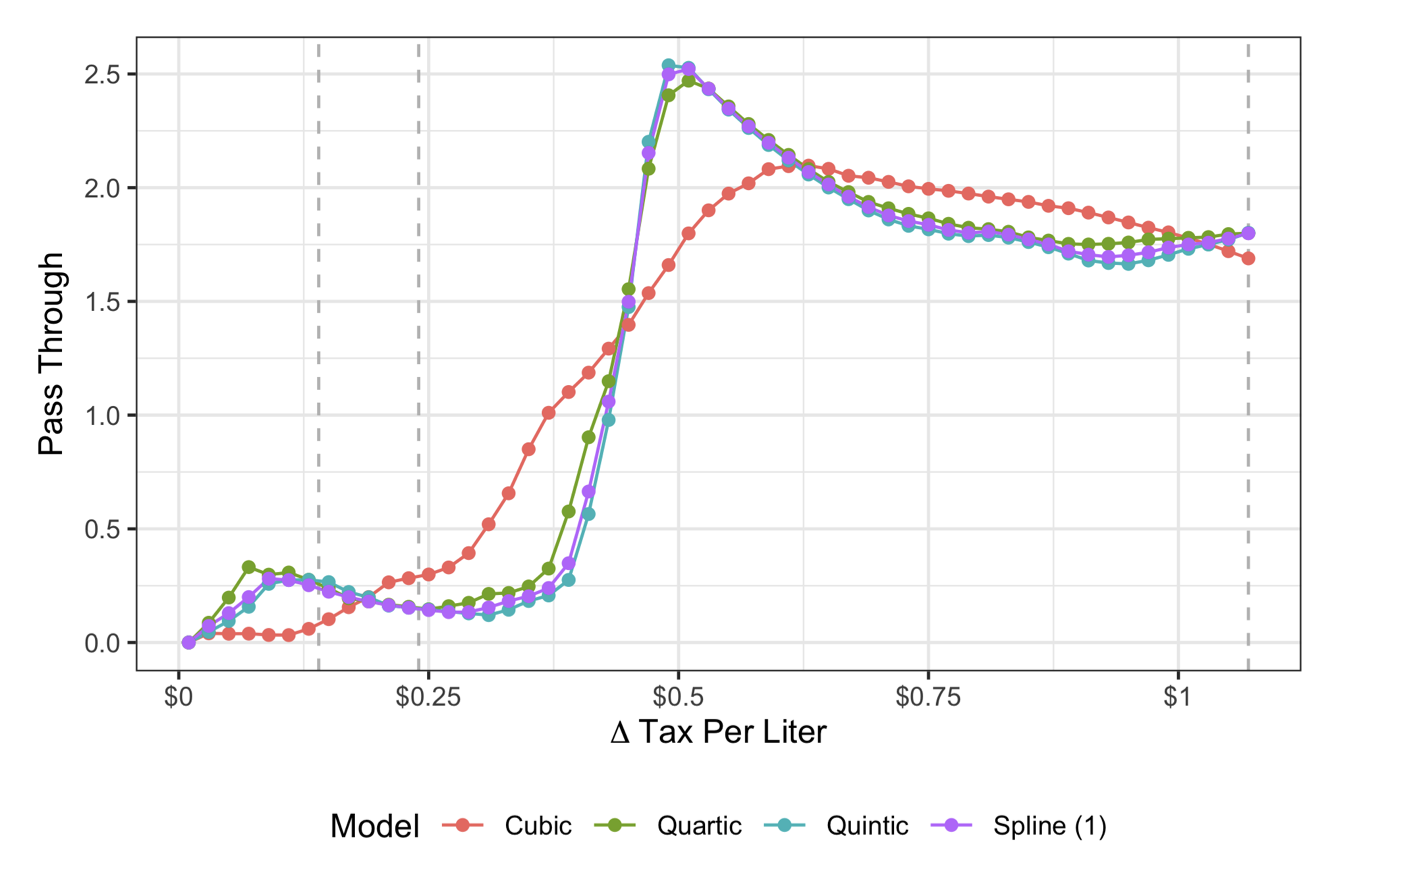
\includegraphics[height=0.8\textheight]{./resources/ptr.png}\\
Cubic isn't flexible enough, spline and quartic look about the same.
\end{center}
\end{frame}



\end{document}